\documentclass[../main.tex]{subfiles}

\begin{document}
	\section{Static Electricity}
		\begin{preamb}
			Static electricity is the study of charges at rest. In this chapter we will explore that very concept.
		\end{preamb}
		
		\pdef{Charge}{Charge is measured in coulombs [\si{\coulomb}]. There are positive and negative charges.}
		Like charges repel, unlike charges attract.
		\begin{center}
			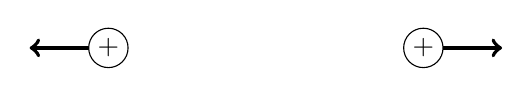
\begin{tikzpicture}
				\draw [line width=0.5mm, ->] (-2,0) -- (-3,0);
				\draw [line width=0.5mm, ->] (2,0) -- (3,0);
				\filldraw [fill=white] (-2,0) circle (0.25) node {\(+\)};
				\filldraw [fill=white] (2,0) circle (0.25) node {\(+\)};
			\end{tikzpicture}
		\end{center}
		\begin{center}
			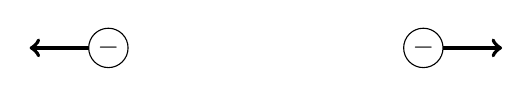
\begin{tikzpicture}
				\draw [line width=0.5mm, ->] (-2,0) -- (-3,0);
				\draw [line width=0.5mm, ->] (2,0) -- (3,0);
				\filldraw [fill=white] (-2,0) circle (0.25) node {\(-\)};
				\filldraw [fill=white] (2,0) circle (0.25) node {\(-\)};
			\end{tikzpicture}
		\end{center}
		\begin{center}
			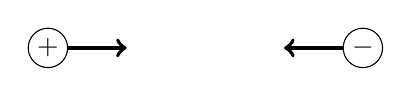
\begin{tikzpicture}
				\draw [line width=0.5mm, ->] (-2,0) -- (-1,0);
				\draw [line width=0.5mm, ->] (2,0) -- (1,0);
				\filldraw [fill=white] (-2,0) circle (0.25) node {\(+\)};
				\filldraw [fill=white] (2,0) circle (0.25) node {\(-\)};
			\end{tikzpicture}
		\end{center}
		
		\subsection{Electric Fields}
		
		\pdef{Electric Field}{An electric field is a region of space whereby a charge experiences an electric force.}
		
		\begin{center}
			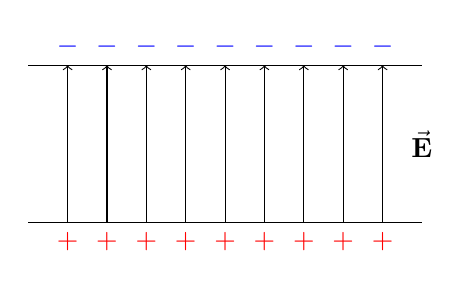
\begin{tikzpicture}
				\foreach \x in {1,...,9}
				\node [color=blue, anchor=south] at (0.5*\x,2) {\(-\)};
				\foreach \x in {1,...,9}
				\node [color=red, anchor=north] at (0.5*\x,0) {\(+\)};
				\node at (5,1) {\(\vec{\mathbf{E}}\)};
				\draw (0,0) -- (5,0);
				\draw (0,2) -- (5,2);
				\foreach \x in {1,...,9}
				\draw [->] (0.5*\x,0) -- (0.5*\x,2);
			\end{tikzpicture}
		\end{center}
		
		\subsubsection{Isolated Charges}
		Field lines are the path a test charge would take within that electric field. The tighter the field lines are, the stronger the electric field at that area, which means that the test charge would experience a stronger force.
		\begin{center}
			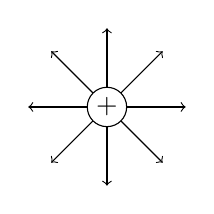
\begin{tikzpicture}
				\foreach \x in {0,...,7}
				\draw [->] (0,0) -- (45*\x:1);
				\filldraw [fill=white] (0,0) circle (0.25) node {\(+\)};				
			\end{tikzpicture}
		\end{center}
		Field lines extend out from positive charges.
		\begin{center}
			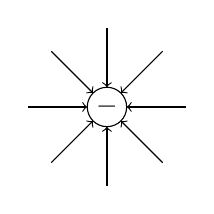
\begin{tikzpicture}
				\foreach \x in {0,...,7}
				\draw [<-] (45*\x:0.25) -- (45*\x:1);
				\filldraw [fill=white] (0,0) circle (0.25) node {\(-\)};				
			\end{tikzpicture}
		\end{center}
		Field lines go in to negative charges.
		
		If a charge is stronger, it gets more field lines (e.g. this one has twice the charge as the one above, so it should get more)
		\begin{center}
			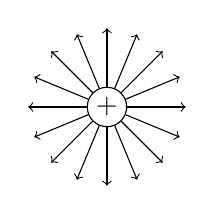
\begin{tikzpicture}
				\foreach \x in {0,...,15}
				\draw [->] (0,0) -- (22.5*\x:1);
				\filldraw [fill=white] (0,0) circle (0.25) node {\(+\)};				
			\end{tikzpicture}
		\end{center}
		
		\subsubsection{Attraction}
		
		\subsubsection{Repulsion}
		
		\subsection{Charging}
\end{document}
